\documentclass[a4paper, 12pt]{article}
\usepackage{graphicx} % Required for inserting images
\usepackage[vietnamese]{babel}
\usepackage[top=1cm, left=1in, right=1in, bottom=2cm]{geometry}
\usepackage{amsfonts, amsmath, amssymb, amsthm}
\usepackage{float}


\title{Mô hình động học phân tử về cấu tạo chất}
\author{Trương Nguyễn Phước Tâm}
\date{2025}

\begin{document}
	
\maketitle

\section{Mô hình động học phân tử về cấu tạo chất}

\raisebox{0.3ex}{\tiny$\bullet$} Các chất được cấu tạo từ các hạt riêng biệt gọi là phân tử.\\
\noindent
\raisebox{0.3ex}{\tiny$\bullet$} Các phân tử chuyển động hỗn loạn không ngừng. Nhiệt độ càng cao thì các phân tử chuyển động càng nhanh.\\
\noindent
\raisebox{0.3ex}{\tiny$\bullet$} Giữa các phân tử có lực hút và lực đẩy gọi chung là lực liên kết phân tử.


\section{Chuyển động của phân tử}
\subsection{Hiện tượng khuếch tán}

\begin{figure}[H]
	\centering
	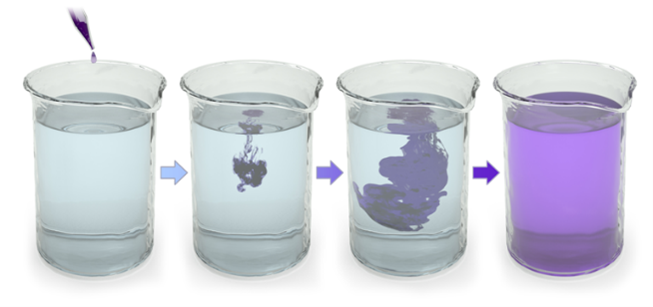
\includegraphics[width=0.3\linewidth]{img/Picture1.png}
	\caption{Hiện tượng khuếch tán}
\end{figure}

Nhỏ một giọt mực vào cốc nước thì xảy ra hiện tượng khuếch tán. Khi cốc nước có nhiệt độ cao hơn thì mực lan nhanh hơn. Hiện tượng khuếch tán không phải do trọng lực hay đối lưu gây ra mà do chuyển động của các phân tử.


\subsection{Chuyển động Brown}

Năm 1827, nhà thực vật học Robert Brown qua sát hạt phân hoa rất nhỏ lơ lửng trong nước bằng kính hiển vi thì thấy chúng chuyển động hỗn loạn không ngừng; nhiệt độ của nước càng cao thì chuyển động của hạt phấn hoa càng nhanh. Ông ghi lại vị trí của hạt phấn hoa sau những khoảng thời gian xác định, rồi nối các điểm đó lại thì thu được một đường gấp khúc không theo trật tự nào. Qua nhiều thí nghiệm, ông còn phát hiện, ngoài hạt phấn hoa, chuyển động này có thể được quan sát ở các hạt khác có kích thước tương tự khi lơ lửng trong chất lỏng. Chuyển động của các hạt lơ lửng trong chất lỏng được gọi là \textbf{chuyển động Brown}.

\begin{figure}[H]
	\centering
	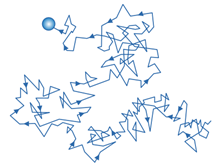
\includegraphics[width=0.2\linewidth]{img/Picture2.png}
	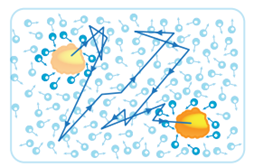
\includegraphics[width=0.2\linewidth]{img/Picture3.png}
	\caption{Thí nghiệm của Brown}
\end{figure}

\textit{Giải thích chuyển động Brown:} Các phân tử nước chuyển động hỗn loạn, không ngừng liên tục va chạm vào hạt phấn hóa. Tại một thời điểm, hạt phấn hoa bị tác động mạnh theo một hướng nhất định; tại thời điểm tiếp theo, hạt phân hoa lại bị tác động mạnh theo một hướng khác nên hướng chuyển động của nó thường xuyên thay đổi.


Nhiệt độ càng cao, các phân tử chuyển động càng nhanh, va đập vào hạt phấn hoa càng mạnh, làm hạt phấn hoa chuyển động càng nhanh. Vì vậy chuyển động không ngừng của các phân tử nước gọi là \textbf{chuyển động nhiệt}. Nhiệt độ là thước đo tốc độ chuyển động nhiệt của phân tử. Vật chất chứa lựng lớn phân tử nên ta quan tâm tới động năng trung bình của các phân tử, nhiệt độ càng cao thì động năng trung bình của các phân tử càng lớn.


\section{Tương tác phân tử}

Chất được cấu tạo từ các phân tử; phân tử gồm hạt nhân mang điện dương và lớp vỏ electron mang điện âm. Hạt nhân hoặc lớp vỏ electron của hai phân tử đẩy nhau, hạt nhân của phân tử này hút lớp vỏ electron của phân tử kia nên giữa các phân tử tồn tại cả lực đẩy và lực hút, gọi là \textbf{lực tương tác (liên kết) giữa các phân tử}.

Ta thấy, khi các phân tử ở gần nhau, chúng có xu hướng đẩy nhau. Khi r tăng, cả lực đẩy và lực hút đều giảm nhưng lực đẩy giảm mạnh hơn nên các phân tử có xu hướng hút nhau. 

\begin{figure}[H]
	\centering
	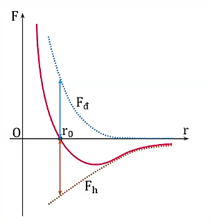
\includegraphics[width=0.3\linewidth]{img/Picture4.png}
	\caption{Đồ thị lực tương tác phân tử}
\end{figure}

\section{Sơ lược về cấu trúc chất rắn, lỏng, khí}
\subsection{Chất rắn}
\raisebox{0.3ex}{\tiny$\bullet$} Các phân tử chất rắn ở rất gần nhau, lực tương tác phân tử rất mạnh.\\
\raisebox{0.3ex}{\tiny$\bullet$} Phân tử chất rắn dao động xung quanh VTCB xác định.\\
\raisebox{0.3ex}{\tiny$\bullet$} Vật rắn có thể tích và hình dạng riêng.\\

\noindent Chất rắn được chia thành 2 loại: chất rắn tinh thể (kết tinh) và chất rắn vô định hình

\textit{Chất rắn tinh thể}: Có cấu trúc tinh thể, các phân tử liên kết chặt với nhau và sắp xếp theo một trật tự hình học xác định, tuần hoàn trong không gian, gọi là mạng tinh thể. Muối ăn, kim  cương, hầu hết kim loại,... là những chất rắn tinh thể.

\begin{figure}[H]
	\centering
	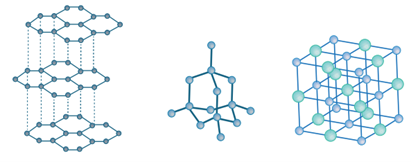
\includegraphics[width=0.5\linewidth]{img/Picture5.png}
	\caption{Đồ thị lực tương tác phân tử}
\end{figure}

\textit{Chất rắn vô định hình}: Không có cấu trúc tinh thể. Thuỷ tinh, nhựa đường, cao su, sô-cô-la,... là những chất rắn vô định hình.

\begin{figure}[H]
	\centering
	
\includegraphics[width=0.5\linewidth]{img/Picture6.png}
	\caption{Đồ thị lực tương tác phân tử}
\end{figure}

\section{Chất khí}
\raisebox{0.3ex}{\tiny$\bullet$} Các phân tử chất khí ở rất xa nhau, tương tác giữa các phân tử rất yếu, hầu như không đáng kể (trừ khi va chạm).\\
\raisebox{0.3ex}{\tiny$\bullet$} Các phân tử chuyển động hỗn loạn, không ngừng về mọi phía.\\
\raisebox{0.3ex}{\tiny$\bullet$} Khối khí không có thể tích và hình dạng riêng mà có thể tích và hình dạng của bình chứa.\\

\section{Chất lỏng}
Chất lỏng là trạng thái trung gian giữa chất rắn và chất khí.

\raisebox{0.3ex}{\tiny$\bullet$} Các phân tử ở xa hơn trong chất rắn nhưng gần hơn trong chất khí nên lực tương tác giữa các phân tử chất lỏng yếu hơn trong chất rắn.

\raisebox{0.3ex}{\tiny$\bullet$} Phân tử chất lỏng dao động xung quanh VTCB có thể dịch chuyển.

\raisebox{0.3ex}{\tiny$\bullet$} Khối lỏng có thể tích riêng và hình dạng của bình chứa.


\end{document}